% !TEX program = pdflatex
% !TEX options = -synctex=1 -interaction=nonstopmode -file-line-error "%DOC%"
% 作业模板
\documentclass[UTF8,10pt,a4paper]{article}
\usepackage{ctex}
\newfontfamily\menlo{MONACO.TTF}
\usepackage{amsmath}
\usepackage{diagbox}
\usepackage{float}
\usepackage{listings}
\usepackage{multirow}
\usepackage{tabularx}

\usepackage{url}
\usepackage{xcolor}
\newcommand{\tabincell}[2]{\begin{tabular}{@{}#1@{}}#2\end{tabular}}

\lstset{
    breaklines,                                 % 自动将长的代码行换行排版
    extendedchars=false,                        % 解决代码跨页时,章节标题,页眉等汉字不显示的问题
    backgroundcolor=\color[rgb]{0.96,0.96,0.96},% 背景颜色
    keywordstyle=\color{blue}\bfseries,         % 关键字颜色
    identifierstyle=\color{black},              % 普通标识符颜色
    commentstyle=\color[rgb]{0,0.6,0},          % 注释颜色
    stringstyle=\color[rgb]{0.58,0,0.82},       % 字符串颜色
    showstringspaces=false,                     % 不显示字符串内的空格
    numbers=left,                               % 显示行号
    numberstyle=\tiny\menlo,                    % 设置数字字体
    basicstyle=\small\menlo,                    % 设置基本字体
    captionpos=t,                               % title在上方(在bottom即为b)
    frame=single,                               % 设置代码框形式
    rulecolor=\color[rgb]{0.8,0.8,0.8},         % 设置代码框颜色
}  

\usepackage{pythonhighlight}
\usepackage{listings}
\usepackage{xcolor}
\usepackage{graphicx}
\usepackage[a4paper,left=2cm,right=2cm,top=2cm,bottom=2cm]{geometry}
\usepackage{fancyhdr}
% \catcode`\。=\active
% \newcommand{。}{.}
\newcommand{\CourseName}{操作系统(Operating System)}
\newcommand{\CourseCode}{CS307 \& CS356}
\newcommand{\Semester}{2020-2021学年第二学期}
\newcommand{\ProjectName} {\Huge{Project 7}} 
\newcommand{\StudentName}{刘涵之}
\newcommand{\StudentID}{519021910102}
\usepackage[vmargin=1in,hmargin=.5in]{geometry}
\usepackage{fancyhdr}
\usepackage{lastpage}
\usepackage{calc}
\pagestyle{fancy}
\fancyhf{}
\fancyhead[L]{\CourseName}
\fancyhead[C]{\ProjectName}
\fancyhead[R]{\StudentName}
\fancyfoot[R]{\thepage\ / \pageref{LastPage}}
\setlength\headheight{12pt}
\fancypagestyle{FirstPageStyle}{
    \fancyhf{}
    \fancyhead[L]{\CourseName\\
        \CourseCode\\
        \Semester}
    \fancyhead[C]{\large\bfseries\ProjectName \\}
    \fancyhead[R]{Name: \makebox[\widthof{\StudentID}][s]{\StudentName}\\
        ID : \StudentID\\
        }
    \fancyfoot[R]{\thepage\ / \pageref{LastPage}}
    \setlength\headheight{36pt}
}
\usepackage{amsmath,amssymb,amsthm,bm}
\allowdisplaybreaks[4]
\newtheoremstyle{Problem}
{}
{}
{}
{}
{\bfseries}
{.}
{ }
{第\thmnumber{ #2}\thmname{ #1}\thmnote{ (#3)} 得分: \underline{\qquad\qquad}}
\theoremstyle{Problem}
\newtheorem{prob}{题}
\newtheoremstyle{Solution}
{}
{}
{}
{}
{\bfseries}
{:}
{ }
{\thmname{#1}}
\makeatletter
\def\@endtheorem{\qed\endtrivlist\@endpefalse}
\makeatother
\theoremstyle{Solution}
\newtheorem*{sol}{解}
\title{Project 7: Contiguous Memory Allocation}
\date{}
% \usepackage{graphicx}
\begin{document}
\maketitle
\thispagestyle{FirstPageStyle}

This project will involve managing a contiguous region of memory of size $MAX$ where address may range from $0 \cdots (MAX - 1)$. This project requires us to respond to four different requests.
\begin{itemize}
  \item Request for a contiguous block of memory;
  \item Release of a contiguous block of memory;
  \item Compact unused holes of memory into one single block;
  \item Report the regions of free and allocated memory.
\end{itemize}

The program will be passed the initial amount of memory at startup, and it will allocate memory using one of the three approaches highlighted in Section 9.2.2, depending on the flag that is passed to \texttt{RQ} commands. The flags are:
\begin{itemize}
  \item \texttt{F}: first-fit;
  \item \texttt{B}: best-fit;
  \item \texttt{W}: worst-fit.
\end{itemize}

This will require the program keep track of the different holes representing available memory. When a request for memory arrives, it will allocate the memory from one of the available holes based on the allocation strategy, It there is insufficient memory to allocate to a request, it will output an error message and reject the request.

The program will also need to keep track of which region of memory has been allocated to which process. This is necessary to support the \texttt{STAT} command and is also needed when memory is released via the \texttt{RL} command, as the process releasing memory is passed to this command. If a partition being released is adjacent to an existing hole, be sure to combine the two holes into a single hole.

If the user enters \texttt{C} command, the program will compact the set of holes into one larger hole. There are several strategies for implementing compaction, one of which is suggested in Section 9.2.3 in textbook. Be sure to update the beginning address of any processes that have been affected by compaction.


\textbf{Design:} My design for this task is:
\begin{itemize}
  \item The linked list is used to present the memory state. I use char \textbf{process} to distinguish the free memory and the allocated memory.
  \item For \texttt{RL} command, \textbf{liner\_compact()} function is used to combine the free memory into one memory block in the linked list.
  \item For \texttt{RQ} command, first-fit, best-fit and worst-fit algorithm are implemented according to the textbook. The basic idea is to traverse the linked list to find the target free memory.
  \item For \texttt{STAT} command, \textbf{output()} function is used to print the current memory state.
  \item For \texttt{C} command, \textbf{compact()} function is used to find all free memory node, delete them from the linked list and add them up to one free memory node.
\end{itemize}

The implementation of the contiguous memory allocator (\texttt{allocator.c}) is shown as follows.
\begin{lstlisting}[language = c ]
#include <stdio.h>
#include <stdlib.h>
#include <unistd.h>
#include <string.h>


struct memory {
    char *process;
    int space;
    struct memory * next;
};

struct memory *head;

void initialize(int space) {
    head = (struct memory *) malloc (sizeof(struct memory));
    head -> process = (char *) malloc (sizeof(char) * 20);
    strcpy(head -> process, "Unused");
    head -> space = space;
    head -> next = NULL;
    return;
}

void output() {
    struct memory *temp = head;
    int address = 0;
    while (temp != NULL) {
        fprintf(stdout, "Addresses [%d:%d] %s\n", address, address + temp -> space - 1, temp -> process);
        address += temp -> space;
        temp = temp -> next;
    }
    return;
}

void liner_compact() {
    struct memory *temp = head;
    while (temp -> next != NULL) {
        struct memory *n = temp -> next;
        if ((strcmp(temp -> process, "Unused") == 0) && (strcmp(n -> process, "Unused") == 0)) {
            temp -> space += n -> space;
            temp -> next = n -> next;
            free(n -> process);
            free(n);
        }else{
            temp = temp -> next;
        }
    }
}

void compact() {
    struct memory *temp = head -> next, *last = head;
    int free_sapce = 0;
    if (temp == NULL) return;
    if (strcmp(head -> process, "Unused") == 0) {
        struct memory *n = head;
        free_sapce += head -> space;
        head = head -> next;
        free(n -> process);
        free(n);
    }
    while (temp != NULL) {
        if (strcmp(temp -> process, "Unused") == 0) {
            free_sapce += temp -> space;
            last -> next = temp -> next;
            free(temp -> process);
            free(temp);
            temp = last -> next;
        } else {
            last = temp;
            temp = temp -> next;
        }
    }
    
    last -> next = (struct memory *) malloc (sizeof(struct memory));
    last = last -> next;
    last -> process = (char *) malloc (sizeof(char) * 20);
    strcpy(last -> process, "Unused");
    last -> space = free_sapce;
    last -> next = NULL;
    return;
}

int main(int argc, char *argv[]) {
	if (argc != 2) {
        fprintf(stdout, "[Error] Wrong input. \n");
        exit(1);
    }
    
    initialize(atoi(argv[1]));

    while (1) {
        char s1[100];
        fprintf(stdout, "allocator>>");
        fscanf(stdin, "%s", s1);
        if (strcmp(s1, "EXIT") == 0) {
            break;
        } else
        if (strcmp(s1, "STAT") == 0) {
            output();
        } else 
        if (strcmp(s1, "RQ") == 0) {
            char process_name[100], mode;
            int process_size;
            fscanf(stdin, "%s %d %c", process_name, &process_size, &mode);
            if (mode == 'F') {
                struct memory *temp = head;
                while (temp != NULL) {
                    if (strcmp(temp -> process, "Unused") == 0) {
                        if (temp -> space > process_size) {
                            struct memory *new = (struct memory *) malloc (sizeof(struct memory));
                            new -> process = (char *) malloc (sizeof(char) * 20);
                            strcpy(new -> process, "Unused");
                            new -> space = temp -> space - process_size;
                            new -> next = temp -> next;

                            strcpy(temp -> process, process_name);
                            temp -> space = process_size;
                            temp -> next = new;
                            
                            break;
                        } else if (temp -> space == process_size) {
                            strcpy(temp -> process, process_name);
                            temp -> space = process_size;

                            break;
                        }
                    }
                    temp = temp -> next;
                }
                if (temp == NULL) {
                    fprintf(stdout, "[Error] Out of Memory, you may need to compact!! \n");
                }
            } else if (mode == 'B') {
                struct memory *temp = head, *target = NULL;
                while (temp != NULL) {
                    if (strcmp(temp -> process, "Unused") == 0) {
                        if (temp -> space >= process_size) {
                            if (target == NULL) {
                                target = temp;
                            } else if (target -> space > temp -> space) {
                                target = temp;
                            }
                        }
                    }
                    temp = temp -> next;
                }
                if (target == NULL) {
                    fprintf(stdout, "[Error] Out of Memory, you may need to compact!! \n");
                } else {
                    if (target -> space > process_size) {
                        struct memory *new = (struct memory *) malloc (sizeof(struct memory));
                        new -> process = (char *) malloc (sizeof(char) * 20);
                        strcpy(new -> process, "Unused");
                        new -> space = target -> space - process_size;
                        new -> next = target -> next;

                        strcpy(target -> process, process_name);
                        target -> space = process_size;
                        target -> next = new;

                        } else if (target -> space == process_size) {
                            strcpy(target -> process, process_name);
                            target -> space = process_size;
                        }
                }
            } else if (mode == 'W') {
                struct memory *temp = head, *target = NULL;
                while (temp != NULL) {
                    if (strcmp(temp -> process, "Unused") == 0) {
                        if (temp -> space >= process_size) {
                            if (target == NULL) {
                                target = temp;
                            } else if (target -> space < temp -> space) {
                                target = temp;
                            }
                        }
                    }
                    temp = temp -> next;
                }
                if (target == NULL) {
                    fprintf(stdout, "[Error] Out of Memory, you may need to compact!! \n");
                } else {
                    if (target -> space > process_size) {
                        struct memory *new = (struct memory *) malloc (sizeof(struct memory));
                        new -> process = (char *) malloc (sizeof(char) * 20);
                        strcpy(new -> process, "Unused");
                        new -> space = target -> space - process_size;
                        new -> next = target -> next;

                        strcpy(target -> process, process_name);
                        target -> space = process_size;
                        target -> next = new;

                        } else if (target -> space == process_size) {
                            strcpy(target -> process, process_name);
                            target -> space = process_size;
                        }
                }
            } else {
                fprintf(stdout, "[Error] Unexpected mode! \n");
            }
        } else
        if (strcmp(s1, "RL") == 0) {
            char process_name[100];
            fscanf(stdin, "%s", process_name);

            struct memory *temp = head;
            while (temp != NULL) {
                if (strcmp(temp -> process, process_name) == 0) {
                    strcpy(temp -> process, "Unused");
                    liner_compact();
                    break;
                }
                temp = temp -> next;
            }
            if (temp == NULL) {
                fprintf(stdout, "[Error] Unexpected Process name! \n");
            }
        } else
        if (strcmp(s1, "C") == 0) {
            compact();
        } else {
            fprintf(stdout, "[Error] Unexpected input! \n");
        }
    }

    return 0;
}
\end{lstlisting}

Makefile for Contiguous Memory Allocation is shown as follow.
\begin{lstlisting}
CC=gcc
CFLAGS=-Wall

all: allocator.o
	$(CC) $(CFLAGS) -o allocator allocator.o

allocator.o: allocator.c
	$(CC) $(CFLAGS) -c allocator.c

clean:
	rm -rf *.o
	rm -rf allocator
\end{lstlisting}



The execution result is shown as follow.

\begin{figure}[H]
    \centering
    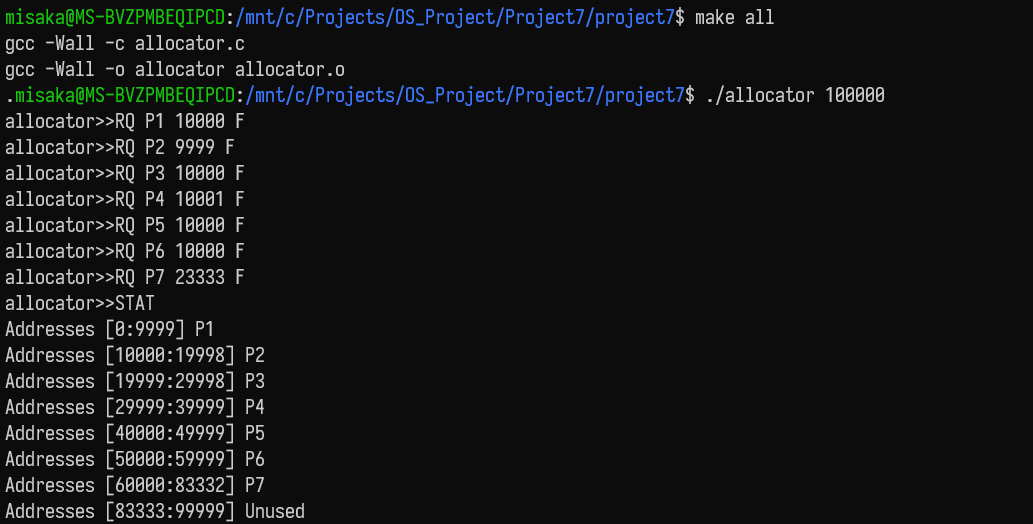
\includegraphics[width=400pt]{1.png}
    \caption{Contiguous Memory Allocation}
    \label{3}
\end{figure}


\begin{figure}[H]
    \centering
    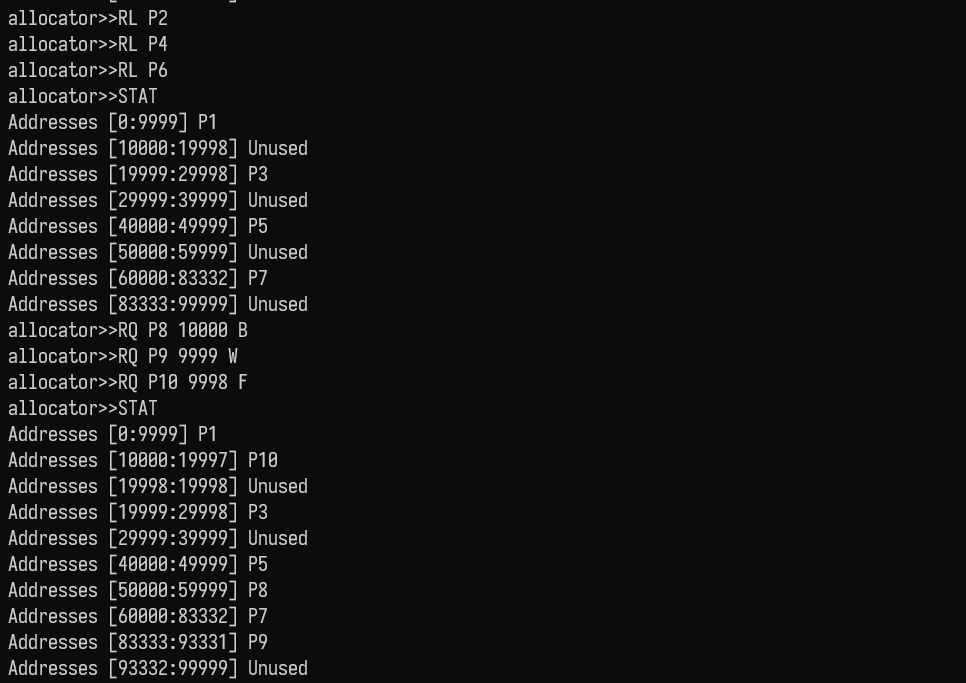
\includegraphics[width=400pt]{2.png}
    \caption{Contiguous Memory Allocation}
    \label{3}
\end{figure}

\begin{figure}[H]
    \centering
    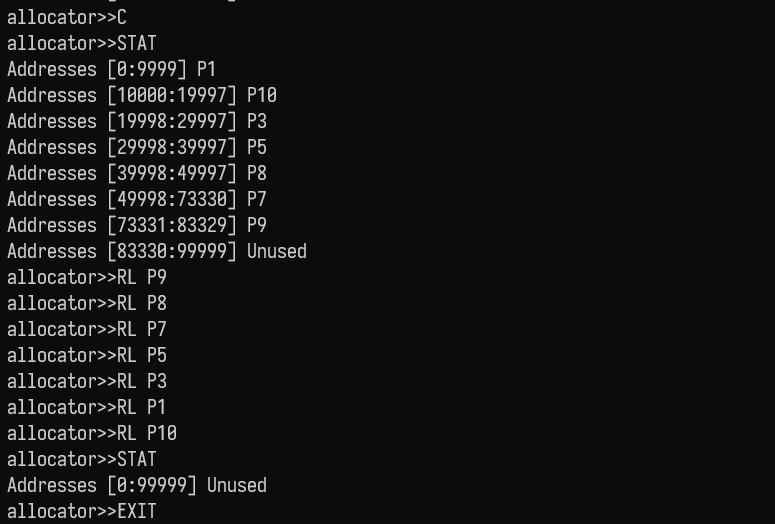
\includegraphics[width=400pt]{3.png}
    \caption{Contiguous Memory Allocation}
    \label{3}
\end{figure}

\end{document}